\documentclass[12pt]{article}
\usepackage[hmargin=1in, vmargin=1in]{geometry}
\usepackage{fancyhdr}
\usepackage{setspace}
\pagestyle{fancy}
\usepackage[small]{caption}
\usepackage{lastpage}
\usepackage{graphicx}
\usepackage{verbatim}
\DeclareGraphicsExtensions{.png}
\usepackage{url}

\def\author{Jacques Uber}
\def\title{Technical Description: FredMeyer Camping Headlamp}
\def\date{\today}

\fancyhf{} % clear all header and footer fields
\fancyhead[LO]{\author}
\fancyhead[RO]{\date}
\renewcommand{\headrulewidth}{0pt}
% The weird spacing here is to get the spacing of \thepage to be right.
\fancyfoot[C]{\thepage\
                    / 4}

\setcounter{secnumdepth}{0}
\setlength{\parindent}{0pt}
\setlength{\parskip}{4mm}
\linespread{1}
% Talk about how the hinge works and where the power switch it relative to how the hinge swings.
% Pictures:
%   Use copyright: Name, Year
% Get rid of value language
%
% OO: Wednesday 9-12
%
\begin{document}
%\fancyhead[CO]{\title}
\begin{center}
\underline{
\large{\title}
}
\end{center}
\begin{comment}
Questions:
*   How should you reference figures and tables in a sentence?
*   What should be in my conclusion?
*   Two or one space after a period?

Introduction:
    "This is what is going on in the paper"

Background:
    "Context" -- Know who your audience is.
    Talk about things outside of the individual object.

Note: You can combine the Into. and Background in this paper.

Body:
    Descriptions of characteristics
    Functions
    Descriptions of related processes

Conclusion:
    "What I need from you"

Formatting
----------
        Title
        -----
Introduction
++++++++++++
Names the object.
Context
Overview
Contents of descriptiong

Body
++++
Characteristics
Components
Materials
Functions

Roby Notes
----------
+ Single spaced
Don't label the table
+ Move title into first page
+ Remove top line
+ Re-work strap paragraph
+ Not "forms of light", "modes" maybe?
+ remove "toggle"-> "pressing the buttom once"
+ Space between units (ie 5 mm)

\end{comment}
\singlespacing
The FredMeyer headlamp is a pocket sized light source made for wearing around a user's head during
situations when visibility could be aided by a supplementary light source.

The headlamp is made up of two physical parts: a black lamp containing 6 LEDs (Light Emitting
Diodes), and a black elastic variable-length strap. The lamp has three settings allowing for light
of different color to be emitted from the LEDs. This paper describes the lamp, strap, and power
settings.

\begin{table}[h!]
\begin{center}
\begin{tabular}{ | c | c | c | p{5cm} |}
    \hline
    Height & Width & Depth \\ \hline
    3.5 cm & 5 cm & 3.5 cm  \\ \hline
\end{tabular}
\end{center}
\caption{Lamp Dimensions. See Figure 3 for spacial orientation.}



\section{The Lamp}
The lamp preforms the primary function of the headlamp. It is 1/4 pounds when loaded with
it's 3 AAA-battery power source. The lamp itself is split into two modules: the bulb housing and the
battery case. The two modules are joined by a hinge which allows the LEDs to be aimed variably (see
Figure 1).

\end{table}
\begin{figure}[h!]
\centering
\caption[Side view of the headlamp] {Side view of the headlamp.}
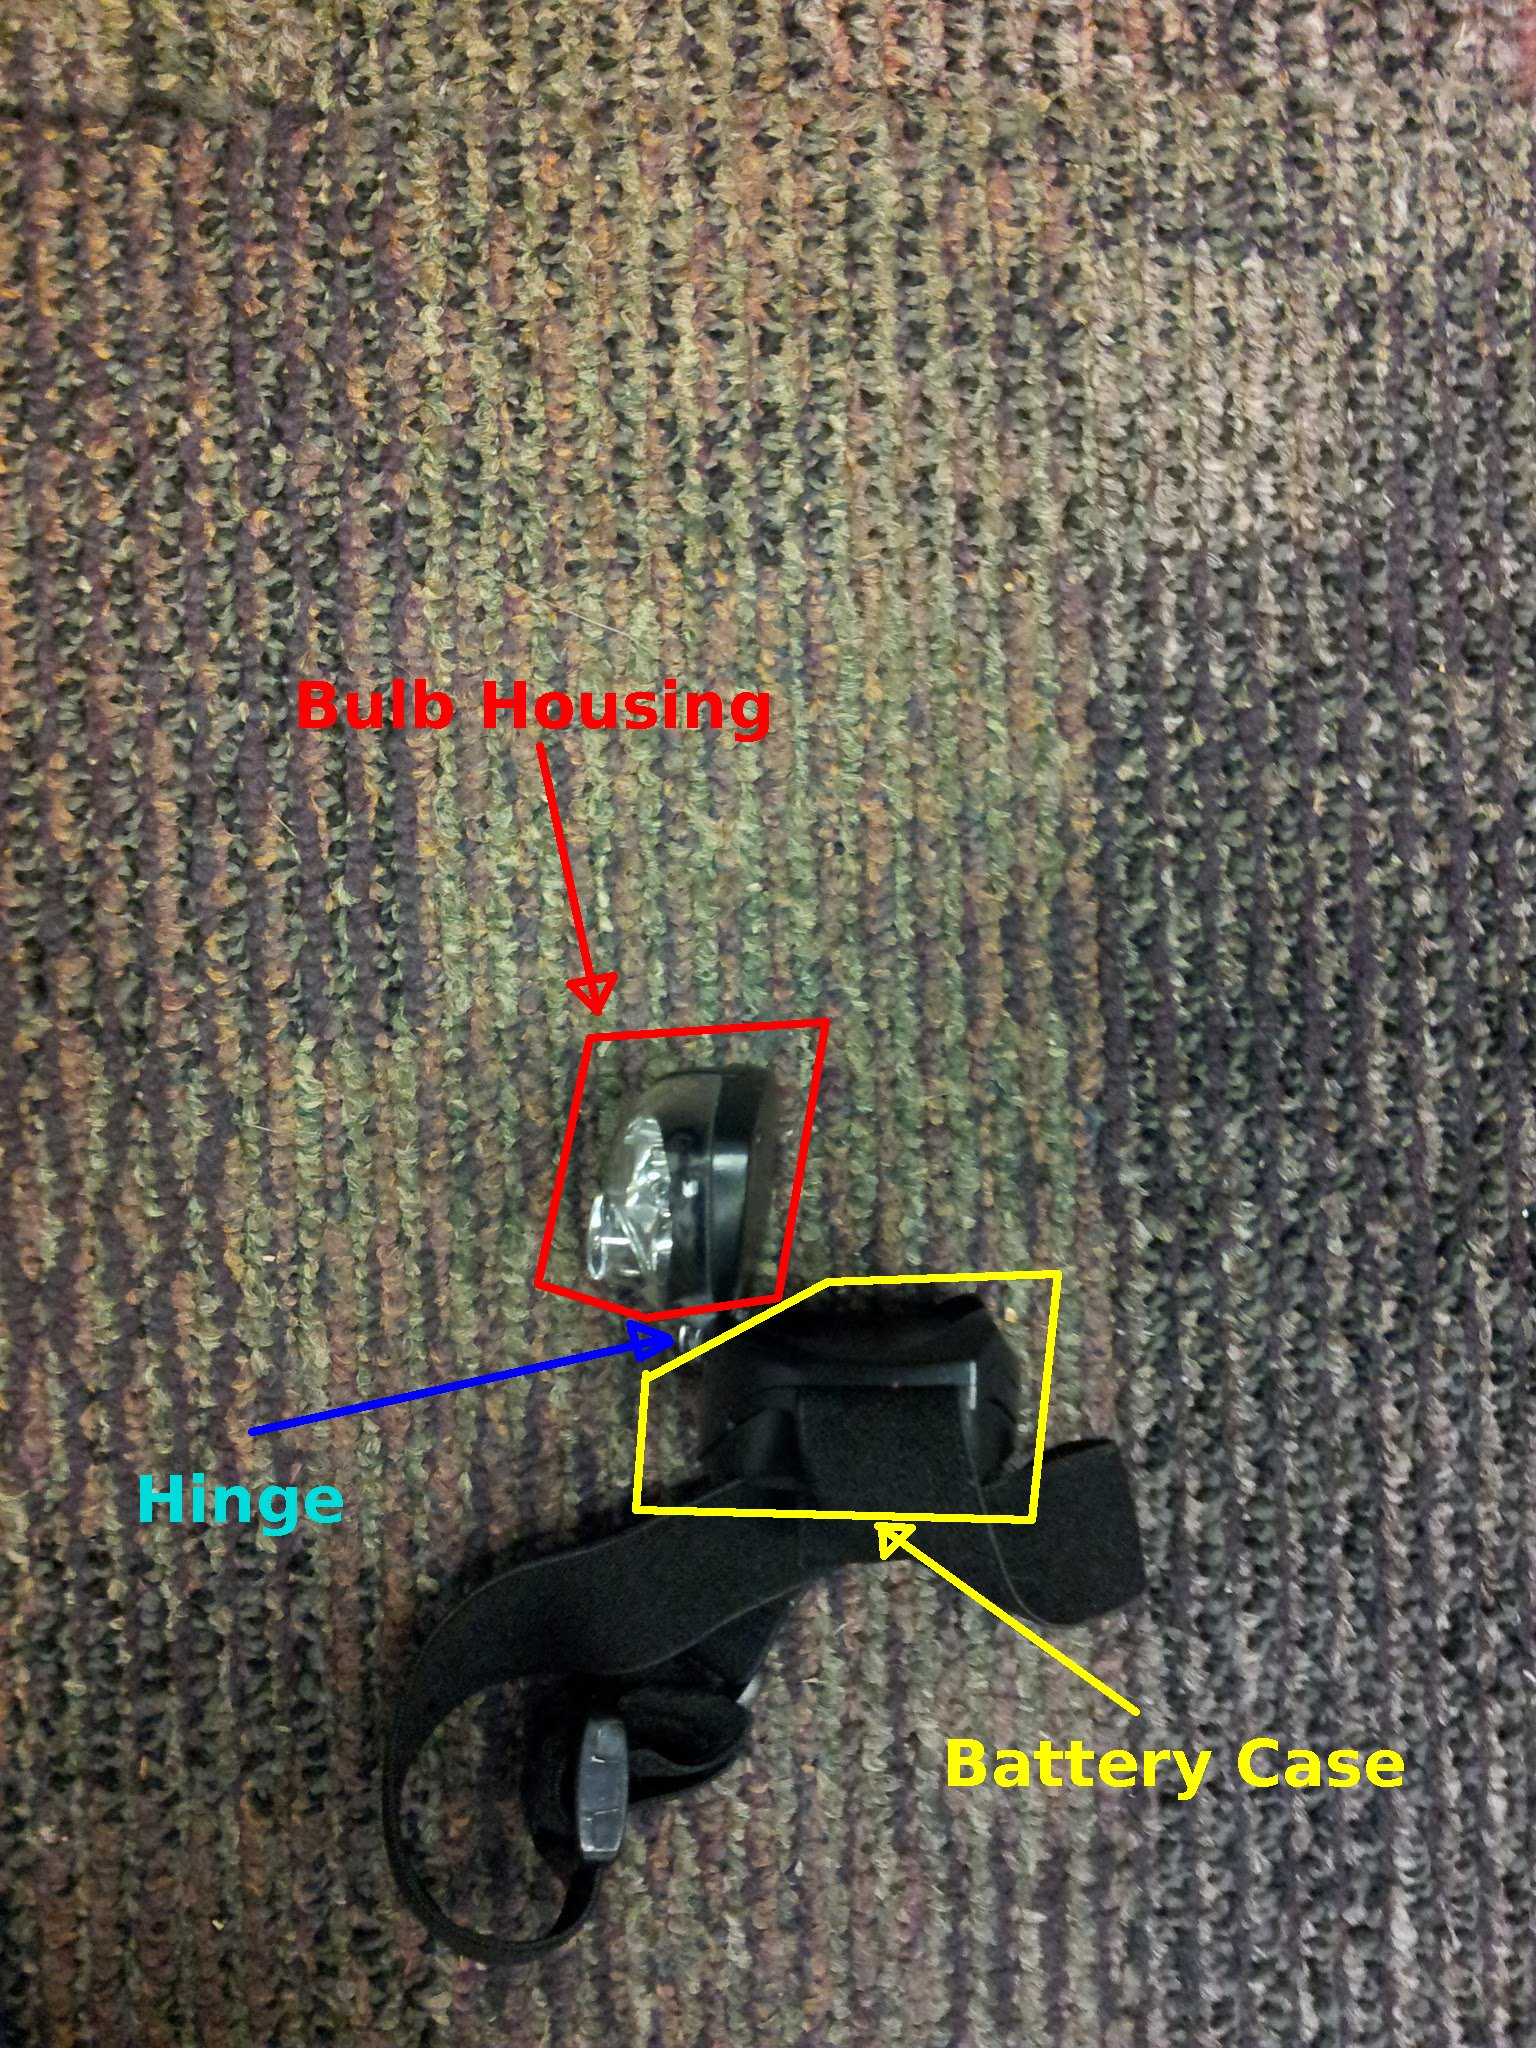
\includegraphics[width=5in]{headlamp_side}
\\ {\tiny \copyright  Jacques Uber 2012}
\end{figure}

\subsection{Bulb Housing}
The bulb housing module holds the LEDs, LED casing, and power switch.

\begin{figure}[h!]
\centering
\label{Figure Derp}
\caption[Front view of the headlamp] {Front view of the headlamp.}
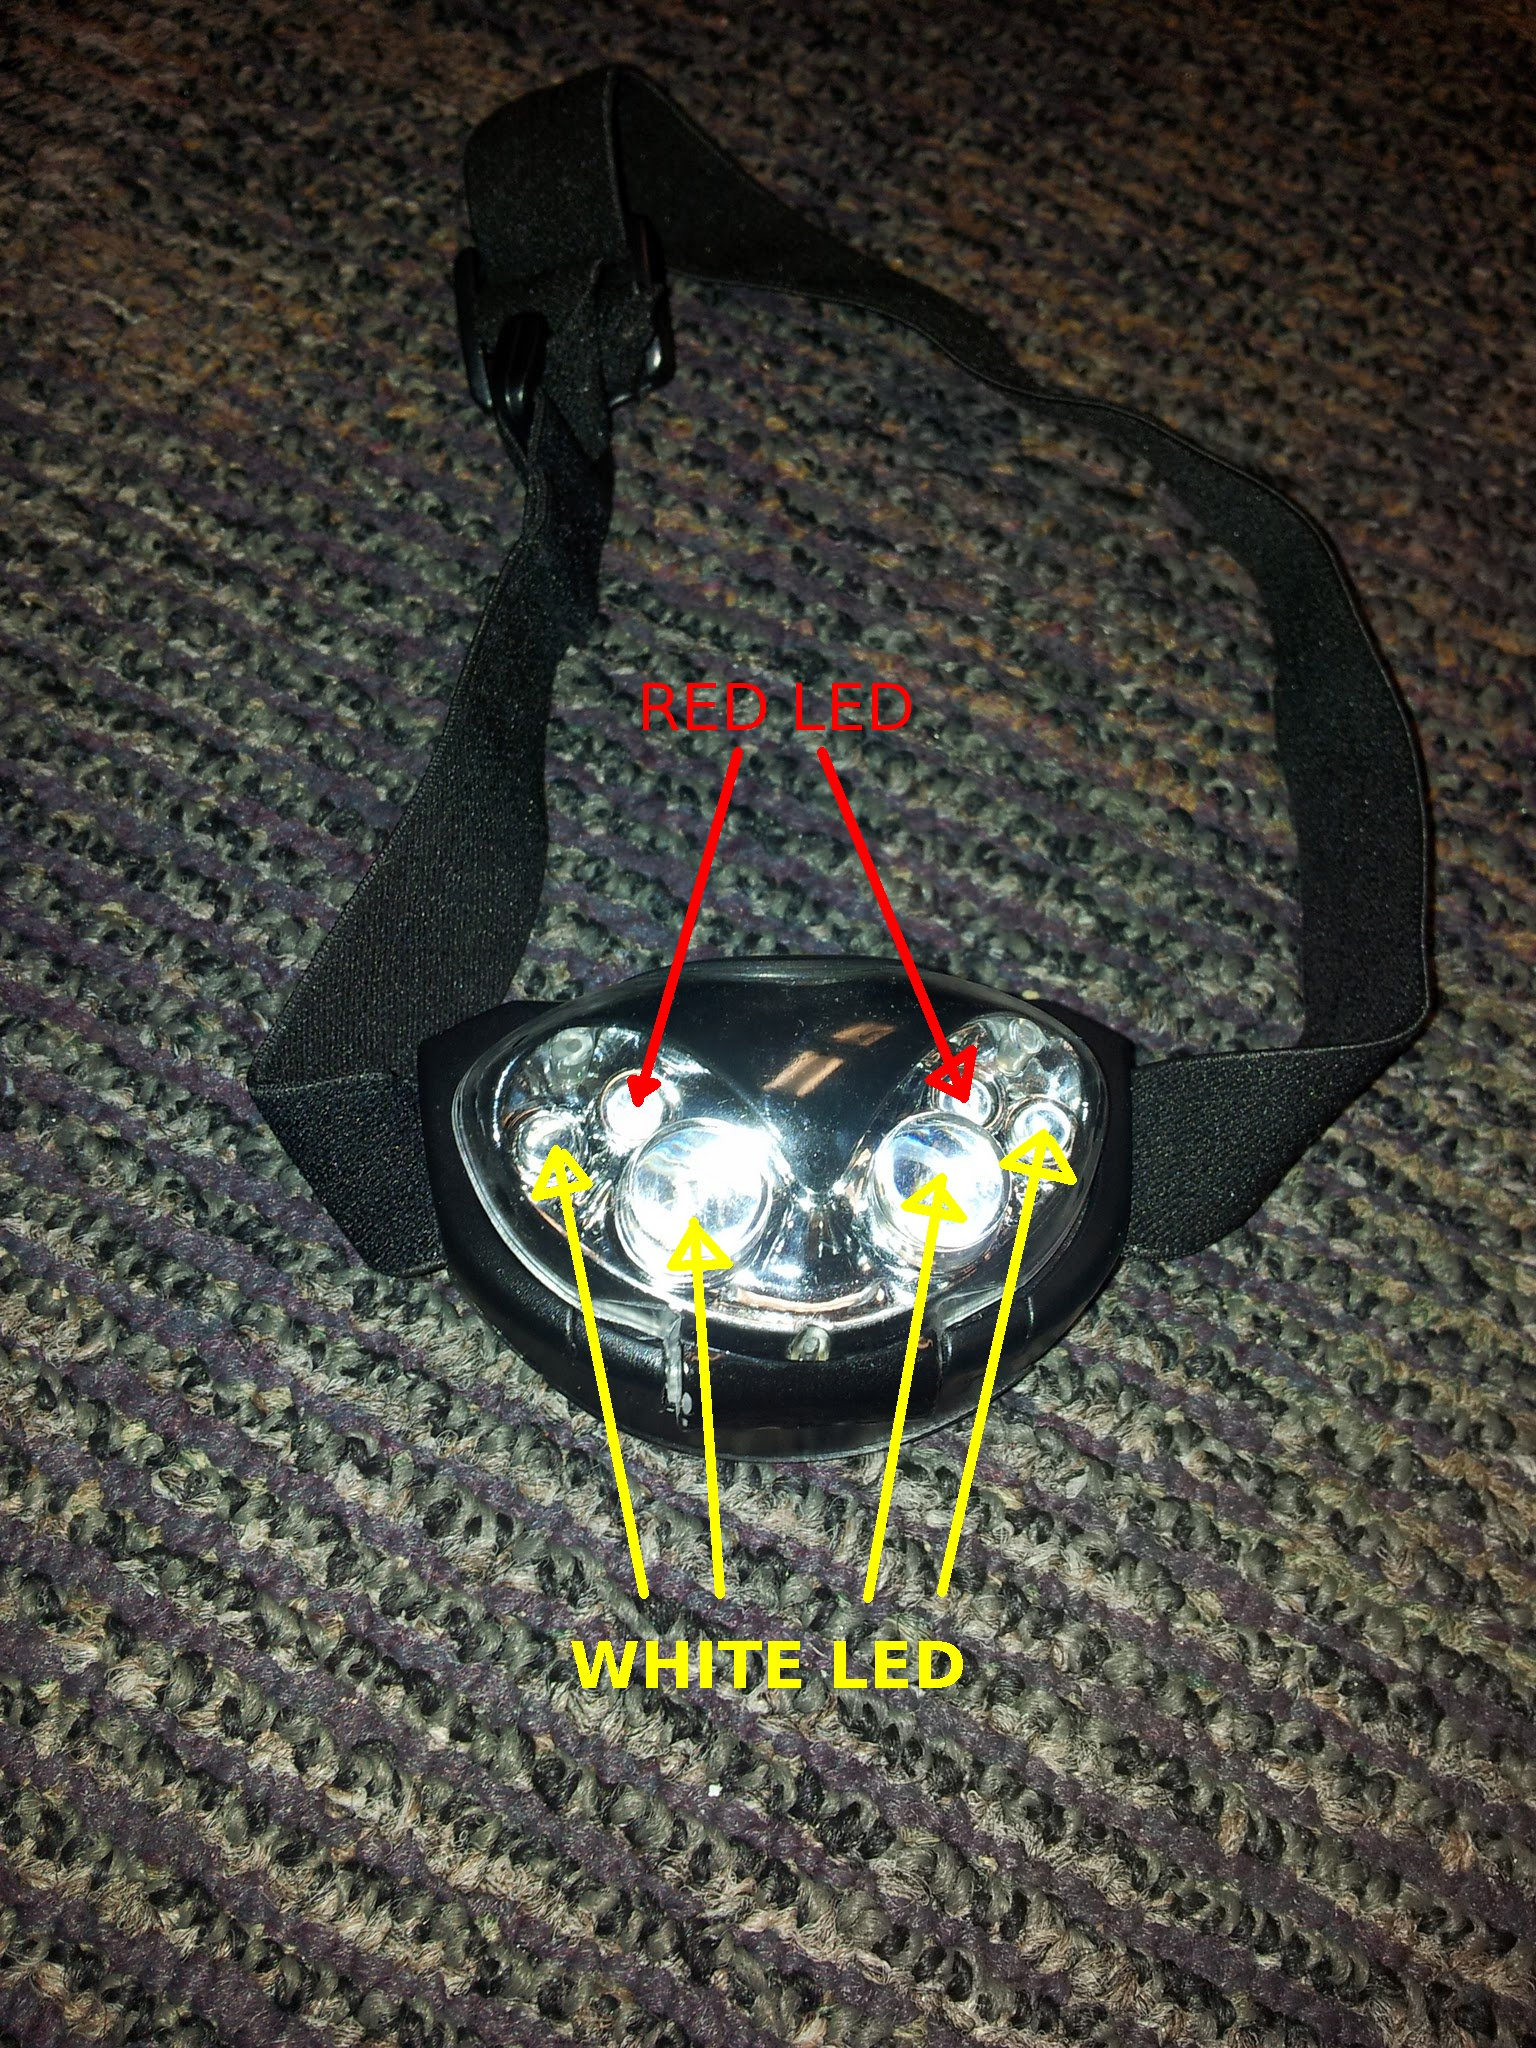
\includegraphics[width=5in]{headlamp}
\\ {\tiny \copyright  Jacques Uber 2012}
\end{figure}

\subsubsection{LEDs}
The lamp has 6 main LEDs, 4 of the LEDs are white and the other 2 are red. Of the 4 white LED's
2 of them have a radius of 0.5 cm and are located symmetrically opposite of each other located 1 cm
away from the front center line of the lamp.  The remaining 4 LEDs have a radius of 0.25 cm and are
aligned symmetrically opposite to each other and are lined up starting 2 cm away from the front
center line of the lamp. With regard to the 4 0.5 cm LEDs, the two furthest from the center line are
white, the inner pair are red (see Figure 2).

\subsubsection{LED Casing}
To protect the LEDs, a clear form fitting case covers the front of the lamp.  The case also acts to
focus and intensify the light from the LEDs. The case consists of hard plastic and is roughly
3 mm thick.

\begin{figure}[h!]
\centering
\caption[Top view of the headlamp] {Top view of the headlamp}
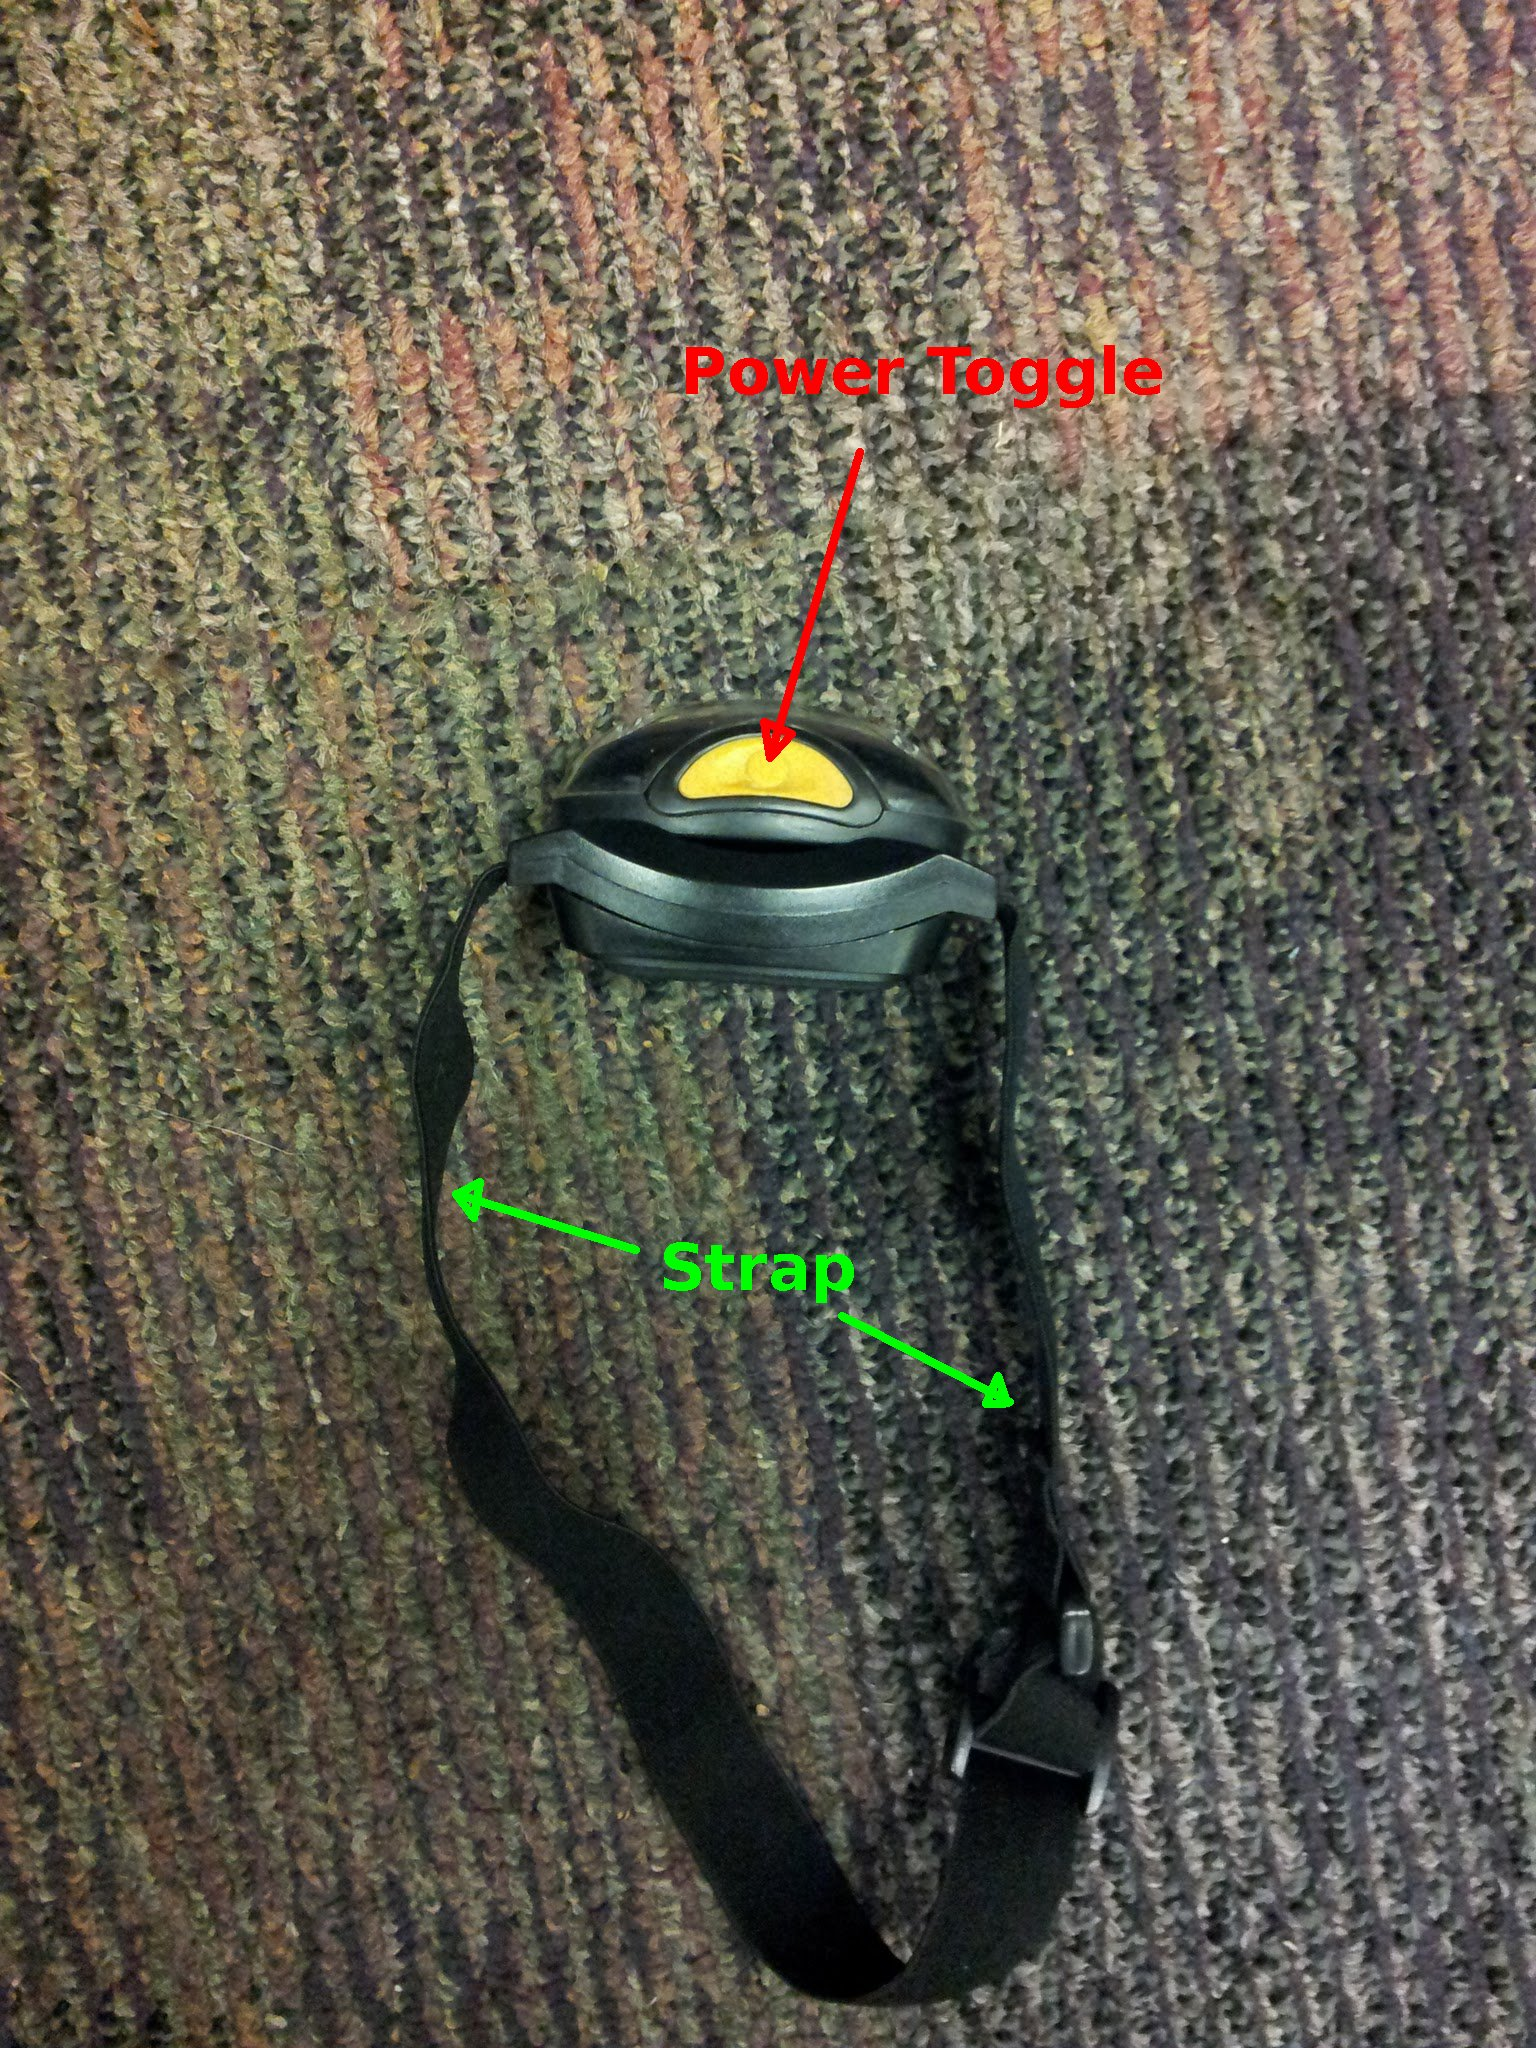
\includegraphics[width=5in]{headlamp_top}
\\ {\tiny \copyright  Jacques Uber 2012}
\end{figure}
\subsubsection{Power button}
Turning on the lamp and cycling through the lamp's power settings is done with the plastic yellow
power button located on the top of the lamp (see Figure 3). The button is pressure sensitive.

\subsection{Battery Case}
The battery case is rectangular with rounded edges (see Figure 1). It is 5 cm across, 3.5 cm wide,
and 1.5 cm deep. When in use, the back of the case is placed onto the users' forehead. To make this
more comfortable there is a soft black pad on the back 5 cm by 3.5 cm panel.

\section{The Strap}
The strap holds the headlamp to the users' head. The elastic variable-length strap is at maximum 2 ft
long, and at minimum 1/2 ft long (see Figure 3).

\section{LED settings}
Pressing the power button will cycle the LEDs through three different modes: Normal-White,
Bright-White, and Flashing-Red (see Table 2). These settings are achieved by powering some LEDs while not
powering others.

\subsection{Normal-White}
From the off state, pressing the button once will place the headlamp into the Normal-White state.  This
setting drives power to the two main 0.5 cm-radius-LEDs.

\subsection{Bright-White}
From the off state, pressing the button twice will place the headlamp into the Bright-White state.
This setting drives power to both the two main 0.5 cm-radius-LEDs and the two outer white 0.25
cm-radius-LEDs. The headlamp emits the most light while in this state.

\subsection{Flashing-Red}
From the off state, pressing the button three times will place the headlamp into the Flashing-Red state.
This setting drives power to the two inner 0.5 cm-radius-LEDs. While in this state the
LEDs will flash on and off at a frequency of 3 times per second. Each flash has a duration of
0.25 seconds.

\begin{table}[h!]
\begin{center}
\begin{tabular}{ | c | c | c | p{5cm} |}
    \hline
    State & State Offset & \# of Powered LEDs & Description \\ \hline
    Normal White & 1 & 2 &  Basic setting. Two main LEDs are powered. Most appropriate for use over
    long durations of time.\\ \hline
    Bright White & 2 & 4 &  Brightest setting. Two main LEDs and two white auxilary LEDs powered.
    Most appropriate setting when a very bright light is needed.\\ \hline
    Flashing Red & 3 & 4 &  Highest contrast setting. Two red auxilary LEDs flash.\\ \hline
\end{tabular}
\end{center}
\caption[Lamp Power States] {Headlamp states. State Offset refers to the offset (number of power
states) from the 'off' state.}
\end{table}

\end{document}
